\section{Rates of Change \& Tangent Lines}
You might already be familiar from physics with the idea of an average rate of change over some interval (often a time interval in physics).
It is simply the amount of change that occurred in the interval, divided by the length of the interval.
This is exactly the same idea as the slope of a line being "rise over run"
\begin{equation*}
	\overline{\Delta f_{a,b}} = \frac{f(b)-f(a)}{b-a}.
\end{equation*}
This is also known as the ``secant slope'', which gets its name from secant lines on circles.

\begin{example}
	Find the average rate of change of $x^2-1$ over the interval $[1,4]$.
\end{example}
\begin{answer}
	Applying the formula,
	\begin{equation*}
		\overline{\Delta f_{1,4}} = \frac{f(4)-f(1)}{4-1} = \frac{15-0}{3} = 5.
	\end{equation*}
\end{answer}

As we decrease the size of the interval, the secant line becomes closer and closer to a tangent line.
In the limit, as the size of the interval approaches 0, we get a tangent line, representing an instantaneous rate of change.
\begin{equation*}
	\Delta f_a = \lim_{h \to 0}{\frac{f(a+h)-f(a)}{h}}.\footnote{You may recognize this from pre-calculus as the ``difference quotient''.}
\end{equation*}

\begin{figure}[H]
	\label{sectant_tangent_line}
	\centering
	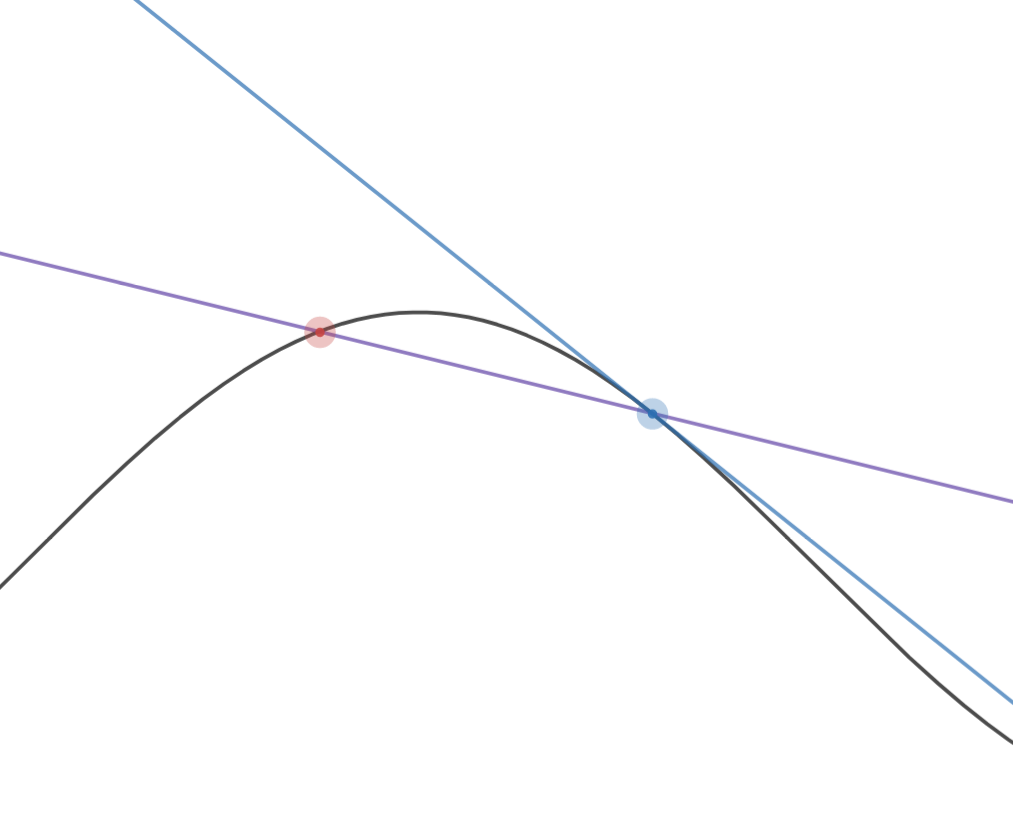
\includegraphics[width = 0.5\textwidth]{./derivatives/secant_tangent_line.png}
	\caption{\hyperref{}{}{}{Secant and Tangent Line}}
\end{figure}

\begin{example}
	Find the equation of the tangent line to $f(x)=x^2-4x$ at $x=1$.
\end{example}
\begin{answer}
	First, we need to find the instantaneous rate of change of $f$ at $x=1$.
	We do this by evaluating the limit.
	\begin{align*}
		\Delta f_{1} &= \lim_{h \to 0}{\frac{f(1+h)-f(1)}{h}} \\
		&= \lim_{h \to 0}{\frac{(1+h)^2-3(1+h) - (1)^2 + 3(1)}{h}} \\
		&= \lim_{h \to 0}{\frac{h^2 + 2h + 1 - 3 - 3h - 1 + 3}{h}} \\
		&= \lim_{h \to 0}{\frac{h^2 - h}{h}} \\
		&= \lim_{h \to 0}{h - 1} \\
		&= -1.
	\end{align*}
	
	Now that we have the slope of the tangent line, we can write the equation of the line in point-slope form.
	We can also rearrange to standard for is needed.
	\begin{align*}
		y - f(1) &= -1(x - 1) \\
		y + 2 &= -x + 1 \\
		y &= -x - 1.
	\end{align*}
\end{answer}